%%%% acra.tex

\typeout{Informative Path Planning with Gaussian Process Classifiers for Seafloor Exploration}

% This is the instructions for authors for ACRA.
\documentclass{article}
\usepackage{acra}
% The file acra.sty is the style file for ACRA. 
% The file named.sty contains macros for named citations as produced 
% by named.bst.

% The preparation of these files was supported by Schlumberger Palo Alto
% Research, AT\&T Bell Laboratories, and Morgan Kaufmann Publishers.
% Shirley Jowell, of Morgan Kaufmann Publishers, and Peter F.
% Patel-Schneider, of AT\&T Bell Laboratories collaborated on their
% preparation. 

% These instructions can be modified and used in other conferences as long
% as credit to the authors and supporting agencies is retained, this notice
% is not changed, and further modification or reuse is not restricted.
% Neither Shirley Jowell nor Peter F. Patel-Schneider can be listed as
% contacts for providing assistance without their prior permission.

% To use for other conferences, change references to files and the
% conference appropriate and use other authors, contacts, publishers, and
% organizations.
% Also change the deadline and address for returning papers and the length and
% page charge instructions.
% Put where the files are available in the appropriate places.


%%%%%% Start: Kelvin's Packages %%%%%% 
\usepackage{vector}  % Allows "\bvec{}" and "\buvec{}" for "blackboard" style bold vectors in maths
\usepackage{bm}
\usepackage{amsmath}
\usepackage{amssymb}
\usepackage{graphicx}
\usepackage[usenames, dvipsnames]{color} % pdfLaTeX
\renewcommand{\vec}[1]{\boldsymbol{#1}}
\newcommand\numberthis{\addtocounter{equation}{1}\tag{\theequation}}

\title{Receding Horizon Approach to Informative Seafloor Exploration using Linearised Entropy of Gaussian Process Classifiers}
% Informative Path Planning with Gaussian Process Classifiers for Seafloor Exploration
% Receding Horizon Approach to Informative Seafloor Exploration with Gaussian Process Classifiers
% Receding Horizon Approach to Informative Seafloor Exploration with Linearised Entropy of Gaussian Process Classifiers

\author{Kelvin Hsu \\ University of Sydney, Australia \\ 
Kelvin.Hsu@nicta.com.au}



\begin{document}

\maketitle

\begin{abstract}
	While seafloor bathymetry have been mapped extensively over the last century, geological and ecological observations of seafloor benthic zones only began recently. Unlike bathymetric mapping, data collection of benthic imagery requires \textit{in situ} exploration - a significantly slower and costly endeavour. An efficient exploration policy would therefore require solving the informative path planning problem. This paper investigates a receding horizon approach to the informative path planning problem using linearised entropy as the proposed acquisition function. We model the benthic environment upon five bathymetric features through Gaussian process classifiers, whose linearised entropy would be defined and derived. We compare our method to a monte carlo approach for estimating joint entropy under a prediction accuracy criterion, demonstrating advantages of the linearised entropy approach. Under the same acquisition criterion, we also show the benefits of a receding horizon approach over simpler approaches such as greedy and open loop methods. Finally, we test our method on collected benthic datasets from past AUV missions to Scott Reef, Western Australia. 
\end{abstract}

\section{Introduction}
\label{Section:Introduction}
	
\section{Background}
\label{Section:Background}

%	\subsection{Laplace Approximation}
%	
%	\subsection{Probabilistic Least Squares}
%	
%	\subsection{Multiclass Classifiers: OVA and AVA approach}
	
\section{Mapping Benthic Habitats with Gaussian Process Classifiers}
\label{Section:BenthicMapping}

	
	
\section{Linearised Entropy of Gaussian Process Classifiers}
\label{Section:LinearisedEntropy}

	\subsection{Binary Classification}
	
		For binary classification, linearisation is performed on the sigmoid, or response, function.
	
		Suppose we have trained our Gaussian process classifier using Laplace approximation with respect to a training set $\mathcal{D} = \{X, \vec{y}\} = \{[ \vec{x}_{1}, \vec{x}_{2}, \dots, \vec{x}_{n}]^{T}, [y_{1}, y_{2}, \dots, y_{n}]\}$ with $n$ training points. We know that the latent function $f(\vec{x})$ is distributed as a GP with a particular predictive mean $m(\vec{x})$ and covariance $k(\vec{x}, \vec{x}')$ once conditioned on the training data \eqref{Section:LinearisedEntropy:Equation:PredictiveGP}.
		
		\begin{equation}
			f(\vec{x}) \sim \mathcal{GP}(m(\vec{x}), k(\vec{x}, \vec{x}'))
		\label{Section:LinearisedEntropy:Equation:PredictiveGP}
		\end{equation}
		
		Let $X^{\star} = [ \vec{x}^{\star}_{1}, \vec{x}^{\star}_{2}, \dots, \vec{x}^{\star}_{n^{\star}}]^{T}$ denote the collection of $n^{\star}$ query points for which inference is to be performed. Denote $\vec{f}^{\star}$ the vector of latent function values $f^{\star}_{i} = f(\vec{x}^{\star}_{i})$ at each query point. We have by definition of a GP that $\vec{f}^{\star}$ is multivariate Gaussian distributed with a corresponding means $\mu^{\star}_{i} = m(\vec{x}^{\star}_{i})$ and covariances $\Sigma^{\star}_{ij} = k(\vec{x}^{\star}_{i}, \vec{x}^{\star}_{j})$ \eqref{Section:LinearisedEntropy:Equation:PredictiveGaussianDistribution}.
		
		\begin{equation}
			\vec{f}^{\star} = [f^{\star}_{1}, f^{\star}_{2}, \dots, f^{\star}_{n^{\star}}]^{T} \sim \mathcal{N}(\vec{\mu}^{\star}, \Sigma^{\star})
		\label{Section:LinearisedEntropy:Equation:PredictiveGaussianDistribution}
		\end{equation}
			
		The binary prediction probability $\vec{\pi^{\star}}$ at the query points is obtained through passing the queried latent function random vector $\vec{f}^{\star}$ through a sigmoid in a component wise fashion \eqref{Section:LinearisedEntropy:Equation:Sigmoid}.
		
		\begin{figure}[!htbp]
			\centering
				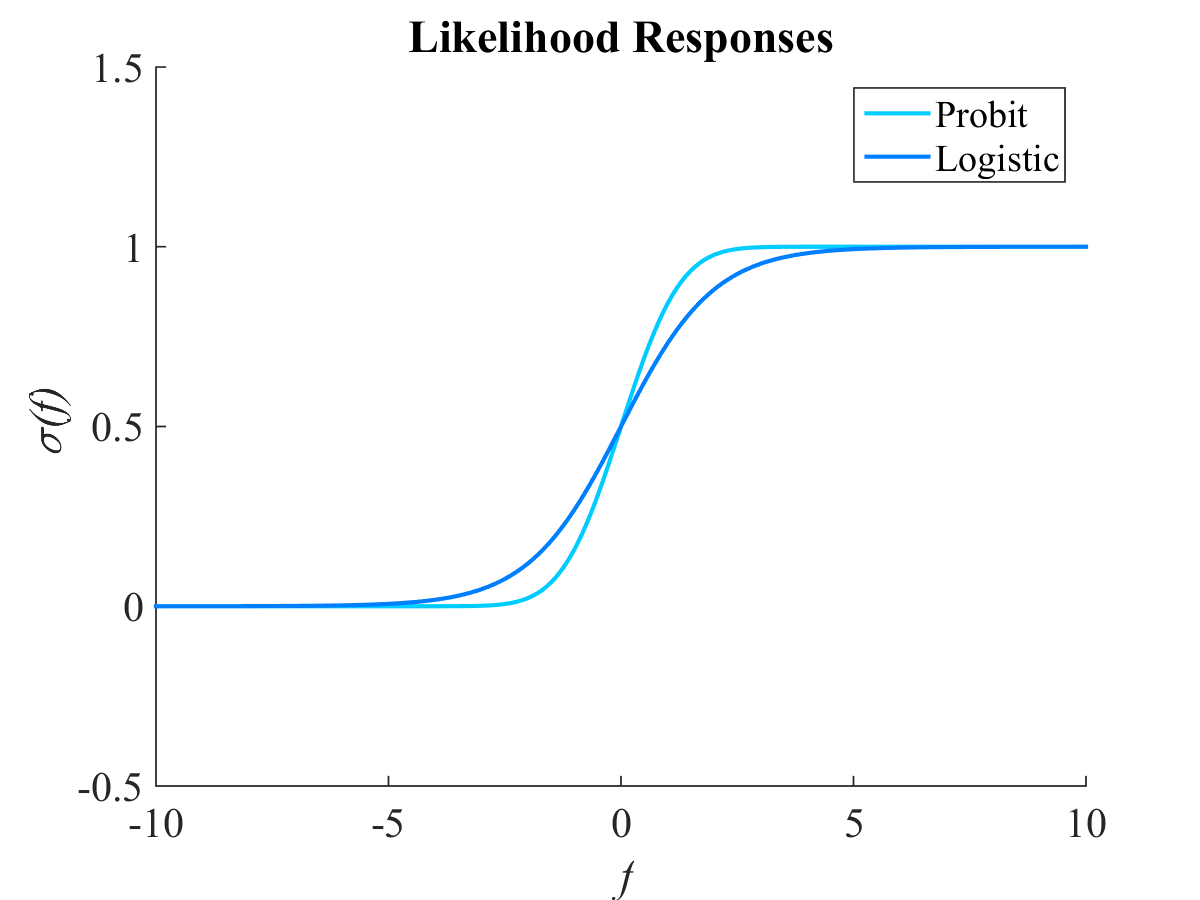
\includegraphics[width=0.48\textwidth]{Figures/responses.png}
			\caption{Likelihood Responses}
			\label{Figure:LikelihoodResponses}
		\end{figure}
		
		\begin{equation}
			\pi^{\star}_{i} = \sigma(f^{\star}_{i}) \qquad \qquad \forall i \in \{1, 2, \dots, n^{\star}\}
		\label{Section:LinearisedEntropy:Equation:Sigmoid}
		\end{equation}
		
		As a straightforward transformation of the latent vector, the predictive probability vector $\vec{\pi^{\star}}$ is thus a random vector itself. The usual procedure is then to treat the expected predition probabilities $\mathbb{E}(\vec{\pi^{\star}})$ as the posterior class probabilities for further inference. However, this discards any information regarding the joint behaviour at the query points. As a result, a measure of mutual information shared amongst the query points cannot be obtained.
		
		One straightforward approach to address this problem is to perform Monte Carlo estimation of the posterior joint distribution for class predictions via jointly sampling latent vectors from the GP and assigning class label 1 for positive latent values and -1 otherwise. Aside from the relatively long computational time required for sampling enough draws for accurate joint distribution estimation, the Monte Carlo approach also has the tendency to overestimate variances at locations of low densities of training observations.

		\begin{figure}[!htbp]
			\centering
				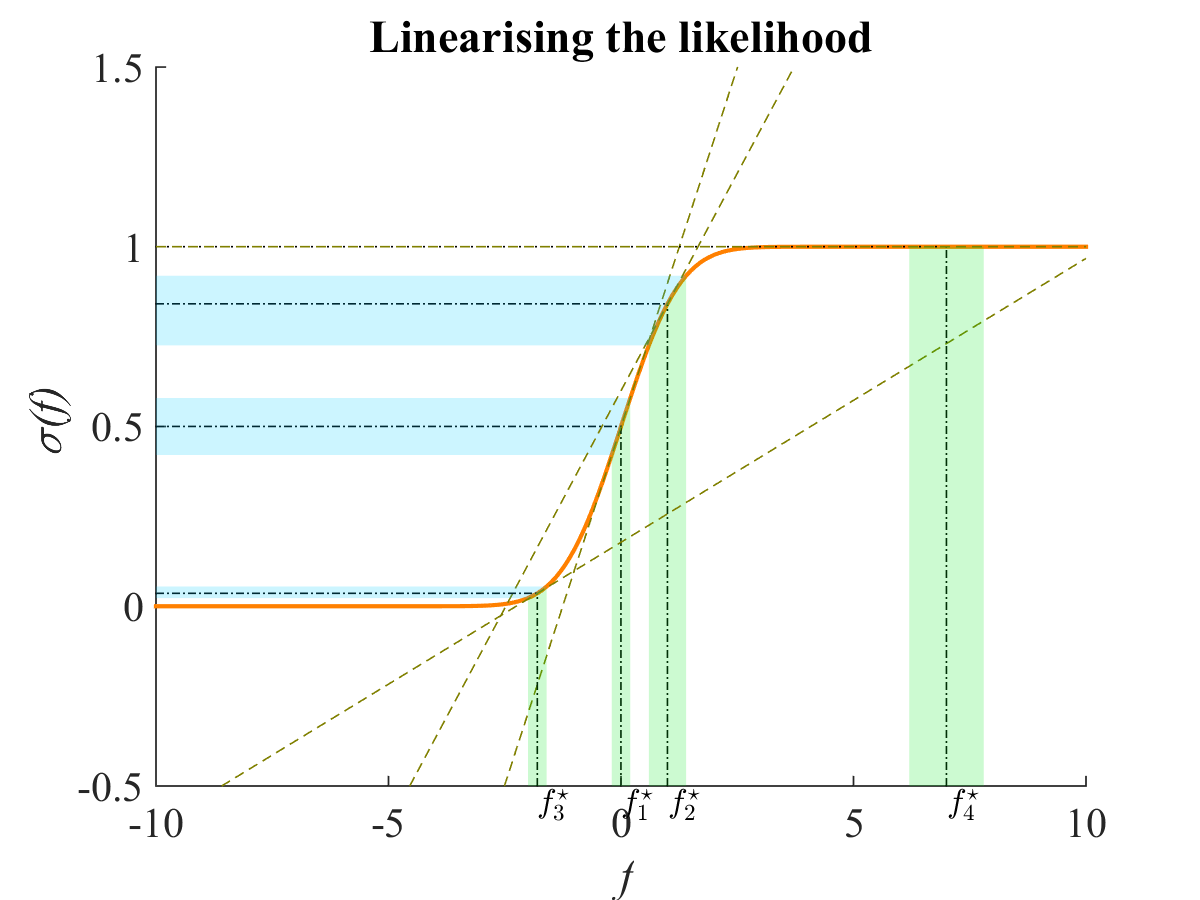
\includegraphics[width=0.48\textwidth]{Figures/linearisation.png}
			\caption{Linearisation Accuracy}
			\label{Figure:Linearisation}
		\end{figure}
				
		Instead, we propose using the joint distribution of the predictive probabilities $\vec{\pi^{\star}}$ itself as a basis of constructing a measure of mutual information. As the predictive probabilities are nonlinear transformations (Figure \ref{Figure:LikelihoodResponses}) of the Gaussian distributed latent vector, they are no longer Gaussian distributed. Nevertheless, there are two situations for which Gaussian approximation through linearised transformations about the mean predictive probabilities would provide accurate estimates:
		
		\begin{enumerate}
			\item $\mathbb{E}(f^{\star}_{i})$ is sufficiently far away from zero
			\item $\mathbb{V}(f^{\star}_{i})$ is sufficiently small
		\end{enumerate}
		
		In fact, when the above two conditions do not hold such that $\mathbb{E}(f^{\star}_{i})$ is close to zero and $\mathbb{V}(f^{\star}_{i})$ is relatively large, we can show that the variances and hence uncertainty estimated from the linearised transformation almost always overestimates the actual variances.

		\subsubsection{Derivation}
		
			We proceed to derive the linearisation which also serves to construct the definition of linearised entropy. Using first order Taylor's expansion, we linearise the sigmoid function about a linearisation point $\bar{f}^{\star}_{i}$ for each query location $i \in \{1, 2, \dots, n^{\star}\}$ \eqref{Section:LinearisedEntropy:Equation:LinearisingSigmoid}. We choose the linearisation point to be the expected latent value at each query point $\bar{f}^{\star}_{i} = \mathbb{E}(f^{\star}_{i})$. 
			
			\begin{equation}
				\sigma(f^{\star}_{i}) \approx \sigma_{L}(f^{\star}_{i}) := \sigma(\bar{f}^{\star}_{i}) + \sigma'(\bar{f}^{\star}_{i}) (f^{\star}_{i} - \bar{f}^{\star}_{i})
			\label{Section:LinearisedEntropy:Equation:LinearisingSigmoid}
			\end{equation}
			
			The prediction probabilities are now approximated as a linear transformation $\sigma_{L}(f)$ of the latent vector, so that it is also multivariate Gaussian distributed with expectance and covariance available in analytical form \eqref{Section:LinearisedEntropy:Equation:MomentsLinearisedSigmoid}.
			
			\begin{align*}
			\numberthis \label{Section:LinearisedEntropy:Equation:MomentsLinearisedSigmoid}
					\sigma_{L}(\vec{f}^{\star}) & \sim \mathcal{N}(\vec{\mu}^{\star}_{L}, \Sigma^{\star}_{L}) \\
					\mathbb{E}(\sigma_{L}(f^{\star}_{i})) & = \mathbb{E}(\sigma(f^{\star}_{i})) = ({\mu^{\star}_{L}})_{i} \\
					\mathbb{C}\mathrm{ov}(\sigma_{L}(f^{\star}_{i}), \sigma_{L}(f^{\star}_{j})) & =  \mathbb{C}\mathrm{ov}(\sigma(\bar{f}^{\star}_{i}) + \sigma'(\bar{f}^{\star}_{i}) (f^{\star}_{i} - \bar{f}^{\star}_{i}),\\ 
					& \qquad \;\;\;\;\; \sigma(\bar{f}^{\star}_{j}) + \sigma'(\bar{f}^{\star}_{j}) (f^{\star}_{j} - \bar{f}^{\star}_{j})) \\
					& = \sigma'(\bar{f}^{\star}_{i}) \sigma'(\bar{f}^{\star}_{j}) \mathbb{C}\mathrm{ov}(f^{\star}_{i}, f^{\star}_{j}) = ({\Sigma^{\star}_{L}})_{ij}			
			\end{align*}
			
			We then define the linearised entropy $H^{\star}_{L}$ at the query points $X^{\star}$ to be the differential entropy for which the random vector $\sigma_{L}(\vec{f}^{\star})$ holds. Since $\sigma_{L}(\vec{f}^{\star})$ is multivariate Gaussian distributed, $H_{L}$ exhibits a closed form \eqref{Section:LinearisedEntropy:Equation:LinearisedEntropy}.
			
			\begin{equation}
				H^{\star}_{L} := \frac{1}{2} \log\Big((2 \pi e)^{n^{\star}} |\Sigma_{L}|\Big)
			\label{Section:LinearisedEntropy:Equation:LinearisedEntropy}
			\end{equation}			
				
		\subsubsection{Properties}
		
			
		
	\subsection{Multiclass Classification}
	
\section{Receding Horizon Approach to Informative Path Planning}
\label{Section:RecedingHorizonApproach}

\section{Conclusions and Future Work}
\label{Section:Conclusion}

\section*{Acknowledgments}


%% This section was initially prepared using BibTeX.  The .bbl file was
%% placed here later
%\bibliography{publications}
%\bibliographystyle{named}
%% The file named.bst is a bibliography style file for BibTeX 0.99c
\begin{thebibliography}{}

\bibitem[\protect\citeauthoryear{Abelson \bgroup \em et al.\egroup
  }{1985}]{abelson-et-al:scheme}
Harold Abelson, Gerald~Jay Sussman, and Julie Sussman.
\newblock {\em Structure and Interpretation of Computer Programs}.
\newblock MIT Press, Cambridge, Massachusetts, 1985.

\bibitem[\protect\citeauthoryear{Brachman and
  Schmolze}{1985}]{brachman-schmolze:kl-one}
Ronald~J. Brachman and James~G. Schmolze.
\newblock An overview of the {KL-ONE} knowledge representation system.
\newblock {\em Cognitive Science}, 9(2):171--216, April--June 1985.

\bibitem[\protect\citeauthoryear{Cheeseman}{1985}]{cheeseman:probability}
Peter Cheeseman.
\newblock In defence of probability.
\newblock In {\em Proceedings of the Ninth International Joint Conference on
  Artificial Intelligence}, pages 1002--1009, Los Angeles, California, August
  1985. International Joint Committee on Artificial Intelligence.

\bibitem[\protect\citeauthoryear{Haugeland}{1981}]{haugeland:mind-design}
John Haugeland, editor.
\newblock {\em Mind Design}.
\newblock Bradford Books, Montgomery, Vermont, 1981.

\bibitem[\protect\citeauthoryear{Lenat}{1981}]{lenat:heuristics}
Douglas~B. Lenat.
\newblock The nature of heuristics.
\newblock Technical Report CIS-12 (SSL-81-1), Xerox Palo Alto Research Centers,
  April 1981.

\bibitem[\protect\citeauthoryear{Levesque}{1984a}]{levesque:functional-foundat%
ions}
Hector~J. Levesque.
\newblock Foundations of a functional approach to knowledge representation.
\newblock {\em Artificial Intelligence}, 23(2):155--212, July 1984.

\bibitem[\protect\citeauthoryear{Levesque}{1984b}]{levesque:belief}
Hector~J. Levesque.
\newblock A logic of implicit and explicit belief.
\newblock In {\em Proceedings of the Fourth National Conference on Artificial
  Intelligence}, pages 198--202, Austin, Texas, August 1984. American
  Association for Artificial Intelligence.

\end{thebibliography}

\end{document}

